\documentclass[conference]{IEEEtran}
\IEEEoverridecommandlockouts

\usepackage[L7x,T1]{fontenc}
\usepackage[utf8]{inputenc}
\usepackage[lithuanian,english]{babel}

% The preceding line is only needed to identify funding in the first footnote. If that is unneeded, please comment it out.
\usepackage{cite}
\usepackage{amsmath,amssymb,amsfonts}
\usepackage{algorithmic}
\usepackage{graphicx}
\usepackage{textcomp}
\usepackage{xcolor}
\def\BibTeX{{\rm B\kern-.05em{\sc i\kern-.025em b}\kern-.08em
    T\kern-.1667em\lower.7ex\hbox{E}\kern-.125emX}}

\usepackage[labelsep=endash]{caption}
\renewcommand{\figurename}{pav}

\usepackage{lipsum}

\begin{document}

\title{Rašytinės LT kalbos identifikavimas (OCR)}

\author{\IEEEauthorblockN{Paulius Milmantas}
\IEEEauthorblockA{\textit{Vilniaus universitetas} \\
\textit{Matematikos ir informatikos fakultetas}\\
Vilnius, Lietuva \\
paulius.milmantas@mif.stud.vu.lt}
}

\maketitle

\begin{abstract}
Santrauka kokia problema spręsta. Ką taikėte, kokie rezultatai.
\end{abstract}

\section{Įvadas}
Užduoties tikslas: parašyti sprendimą, kuris iš duotos
nuotraukos išgautų joje pateiktą Lietuvišką rašytinį tekstą.

\section{Metodai}

\subsection{Taikyta nuostolių funkcija}

Darbe buvo naudota MSE (Mean Square Error) funkcija. ~\eqref{eq:lygtis1}

\begin{equation}
MSE = \frac{1}{n} * \sum_{i=1}^{n} (y_{i} - y_{i}^{p})^{2}
\label{eq:lygtis1}
\end{equation}

\subsection{Optimizavimo funkcija}

Optimizavimui buvo naudota stachastinio gradientinio nuolydžio
(SGD) optimizavimo funckija. ~\eqref{eq:lygtis2}

\begin{equation}
\theta^{(\tau)} = \theta^{(\tau - 1)} - \eta * \bigtriangledown_{\theta} Loss(\theta^{(\tau - 1)};(x_{i}, y_{i}))
\label{eq:lygtis2}
\end{equation}

\subsection{Naudojamas tinklas}

Visos abėcėlės raidės yra suskirstomos į poaibius po 3 raides. ~\ref{fig1} Kiekvienam poaibiui yra
sukuriama po atskirą neuroninį tinklą. Taip yra lengviau atlinkti tinklo treniravimą
ir tinklo užkrovimui galima sutaupyti RAM atminties. Norint pridėti daugiau
duomenų, užtenka tinklą apmokyti tik vienam naujam poaibiui.
\par
Tinklą sudaro 2 paslėpti sluoksniai, 1 įvesties ir 1 išvesties sluoksnis. Duomenys
yra 64x64 dydžio pilki vaizdai, todėl įvesties sluoksnis yra 4096 dydžio. Išvesties
sluoksnis yra 3 dydžio, nes visi poaibiai yra sudaryti iš 3 narių. Visi sluoksniai naudoja
RELU akvytavijos funkcijas.

\begin{figure}[!h] % įterpti čia
\centerline{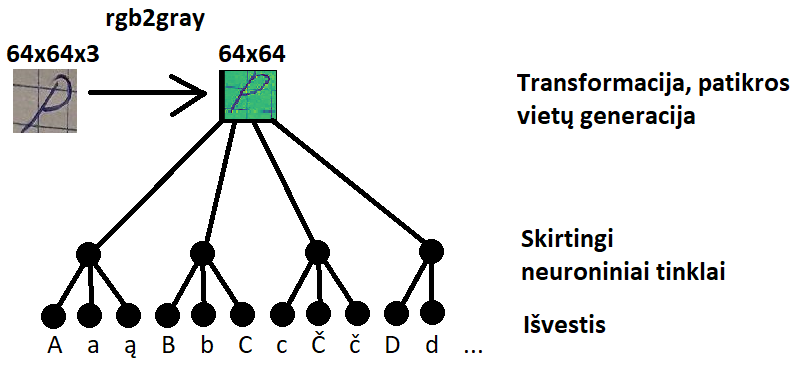
\includegraphics[scale=0.4] {images/1.png}}
\caption{Tinklo sudėtis.}
\label{fig1}
\end{figure}

\subsection{Vaizdo apdorojimas}

\section{Duomenys}

Sužymėtų duomenų, kurių reikia norint išmokyti modelį, internete nėra, todėl
jie buvo renkami ranka. Ant lapo buvo surašomos raidės ir visas lapas buvo
nufotografuojamas. Gautos fotografijos buvo apdorojamos duomenų žymėjimo programa,
kuri kaip rezultatą eksportavo JSON formato failą su kiekvienos raidės pozicija
nuotraukoje. Pagal gautą JSON failą kiekviena raidė buvo eksportuota į atskirą JPG
failą ir atitinkamai apdorota: naudojant nearest neighbour metodą sumažinta iki
64x64 dydžio ir panaikintas RGB kanalas.


\section{Rezultatai}

\begin{figure*}[ht] % puslapio viršuje
\centerline{
\includegraphics{fig1.png}}
\caption{Paveikslėlio aprašas.}
\label{fig}
\end{figure*}


\lipsum[2-10]






Cituojame šaltinį \cite{lecun2015deep}.

\bibliographystyle{plain}
\bibliography{saltiniai}

\end{document}
